\documentclass[1p]{elsarticle_modified}
%\bibliographystyle{elsarticle-num}

%\usepackage[colorlinks]{hyperref}
%\usepackage{abbrmath_seonhwa} %\Abb, \Ascr, \Acal ,\Abf, \Afrak
\usepackage{amsfonts}
\usepackage{amssymb}
\usepackage{amsmath}
\usepackage{amsthm}
\usepackage{scalefnt}
\usepackage{amsbsy}
\usepackage{kotex}
\usepackage{caption}
\usepackage{subfig}
\usepackage{color}
\usepackage{graphicx}
\usepackage{xcolor} %% white, black, red, green, blue, cyan, magenta, yellow
\usepackage{float}
\usepackage{setspace}
\usepackage{hyperref}

\usepackage{tikz}
\usetikzlibrary{arrows}

\usepackage{multirow}
\usepackage{array} % fixed length table
\usepackage{hhline}

%%%%%%%%%%%%%%%%%%%%%
\makeatletter
\renewcommand*\env@matrix[1][\arraystretch]{%
	\edef\arraystretch{#1}%
	\hskip -\arraycolsep
	\let\@ifnextchar\new@ifnextchar
	\array{*\c@MaxMatrixCols c}}
\makeatother %https://tex.stackexchange.com/questions/14071/how-can-i-increase-the-line-spacing-in-a-matrix
%%%%%%%%%%%%%%%

\usepackage[normalem]{ulem}

\newcommand{\msout}[1]{\ifmmode\text{\sout{\ensuremath{#1}}}\else\sout{#1}\fi}
%SOURCE: \msout is \stkout macro in https://tex.stackexchange.com/questions/20609/strikeout-in-math-mode

\newcommand{\cancel}[1]{
	\ifmmode
	{\color{red}\msout{#1}}
	\else
	{\color{red}\sout{#1}}
	\fi
}

\newcommand{\add}[1]{
	{\color{blue}\uwave{#1}}
}

\newcommand{\replace}[2]{
	\ifmmode
	{\color{red}\msout{#1}}{\color{blue}\uwave{#2}}
	\else
	{\color{red}\sout{#1}}{\color{blue}\uwave{#2}}
	\fi
}

\newcommand{\Sol}{\mathcal{S}} %segment
\newcommand{\D}{D} %diagram
\newcommand{\A}{\mathcal{A}} %arc


%%%%%%%%%%%%%%%%%%%%%%%%%%%%%5 test

\def\sl{\operatorname{\textup{SL}}(2,\Cbb)}
\def\psl{\operatorname{\textup{PSL}}(2,\Cbb)}
\def\quan{\mkern 1mu \triangleright \mkern 1mu}

\theoremstyle{definition}
\newtheorem{thm}{Theorem}[section]
\newtheorem{prop}[thm]{Proposition}
\newtheorem{lem}[thm]{Lemma}
\newtheorem{ques}[thm]{Question}
\newtheorem{cor}[thm]{Corollary}
\newtheorem{defn}[thm]{Definition}
\newtheorem{exam}[thm]{Example}
\newtheorem{rmk}[thm]{Remark}
\newtheorem{alg}[thm]{Algorithm}

\newcommand{\I}{\sqrt{-1}}
\begin{document}

%\begin{frontmatter}
%
%\title{Boundary parabolic representations of knots up to 8 crossings}
%
%%% Group authors per affiliation:
%\author{Yunhi Cho} 
%\address{Department of Mathematics, University of Seoul, Seoul, Korea}
%\ead{yhcho@uos.ac.kr}
%
%
%\author{Seonhwa Kim} %\fnref{s_kim}}
%\address{Center for Geometry and Physics, Institute for Basic Science, Pohang, 37673, Korea}
%\ead{ryeona17@ibs.re.kr}
%
%\author{Hyuk Kim}
%\address{Department of Mathematical Sciences, Seoul National University, Seoul 08826, Korea}
%\ead{hyukkim@snu.ac.kr}
%
%\author{Seokbeom Yoon}
%\address{Department of Mathematical Sciences, Seoul National University, Seoul, 08826,  Korea}
%\ead{sbyoon15@snu.ac.kr}
%
%\begin{abstract}
%We find all boundary parabolic representation of knots up to 8 crossings.
%
%\end{abstract}
%\begin{keyword}
%    \MSC[2010] 57M25 
%\end{keyword}
%
%\end{frontmatter}

%\linenumbers
%\tableofcontents
%
\newcommand\colored[1]{\textcolor{white}{\rule[-0.35ex]{0.8em}{1.4ex}}\kern-0.8em\color{red} #1}%
%\newcommand\colored[1]{\textcolor{white}{ #1}\kern-2.17ex	\textcolor{white}{ #1}\kern-1.81ex	\textcolor{white}{ #1}\kern-2.15ex\color{red}#1	}

{\Large $\underline{12n_{0068}~(K12n_{0068})}$}

\setlength{\tabcolsep}{10pt}
\renewcommand{\arraystretch}{1.6}
\vspace{1cm}\begin{tabular}{m{100pt}>{\centering\arraybackslash}m{274pt}}
\multirow{5}{120pt}{
	\centering
	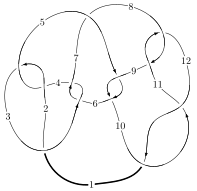
\includegraphics[width=112pt]{../../../GIT/diagram.site/Diagrams/png/2157_12n_0068.png}\\
\ \ \ A knot diagram\footnotemark}&
\allowdisplaybreaks
\textbf{Linearized knot diagam} \\
\cline{2-2}
 &
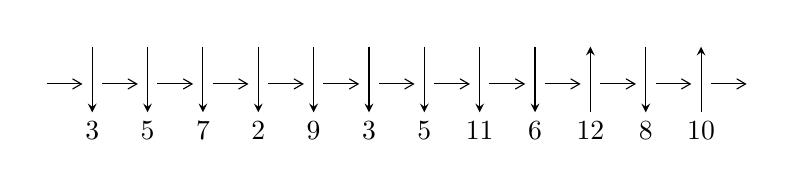
\begin{tikzpicture}[x=20pt, y=17pt]
	% nodes
	\node (C0) at (0, 0) {};
	\node (C1) at (1, 0) {};
	\node (C1U) at (1, +1) {};
	\node (C1D) at (1, -1) {3};

	\node (C2) at (2, 0) {};
	\node (C2U) at (2, +1) {};
	\node (C2D) at (2, -1) {5};

	\node (C3) at (3, 0) {};
	\node (C3U) at (3, +1) {};
	\node (C3D) at (3, -1) {7};

	\node (C4) at (4, 0) {};
	\node (C4U) at (4, +1) {};
	\node (C4D) at (4, -1) {2};

	\node (C5) at (5, 0) {};
	\node (C5U) at (5, +1) {};
	\node (C5D) at (5, -1) {9};

	\node (C6) at (6, 0) {};
	\node (C6U) at (6, +1) {};
	\node (C6D) at (6, -1) {3};

	\node (C7) at (7, 0) {};
	\node (C7U) at (7, +1) {};
	\node (C7D) at (7, -1) {5};

	\node (C8) at (8, 0) {};
	\node (C8U) at (8, +1) {};
	\node (C8D) at (8, -1) {11};

	\node (C9) at (9, 0) {};
	\node (C9U) at (9, +1) {};
	\node (C9D) at (9, -1) {6};

	\node (C10) at (10, 0) {};
	\node (C10U) at (10, +1) {};
	\node (C10D) at (10, -1) {12};

	\node (C11) at (11, 0) {};
	\node (C11U) at (11, +1) {};
	\node (C11D) at (11, -1) {8};

	\node (C12) at (12, 0) {};
	\node (C12U) at (12, +1) {};
	\node (C12D) at (12, -1) {10};
	\node (C13) at (13, 0) {};

	% arrows
	\draw[->,>={angle 60}]
	(C0) edge (C1) (C1) edge (C2) (C2) edge (C3) (C3) edge (C4) (C4) edge (C5) (C5) edge (C6) (C6) edge (C7) (C7) edge (C8) (C8) edge (C9) (C9) edge (C10) (C10) edge (C11) (C11) edge (C12) (C12) edge (C13) ;	\draw[->,>=stealth]
	(C1U) edge (C1D) (C2U) edge (C2D) (C3U) edge (C3D) (C4U) edge (C4D) (C5U) edge (C5D) (C6U) edge (C6D) (C7U) edge (C7D) (C8U) edge (C8D) (C9U) edge (C9D) (C10D) edge (C10U) (C11U) edge (C11D) (C12D) edge (C12U) ;
	\end{tikzpicture} \\
\hhline{~~} \\& 
\textbf{Solving Sequence} \\ \cline{2-2} 
 &
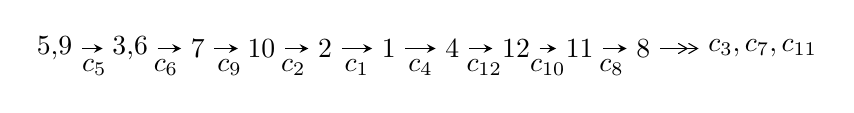
\begin{tikzpicture}[x=23pt, y=7pt]
	% node
	\node (A0) at (-1/8, 0) {5,9};
	\node (A1) at (17/16, 0) {3,6};
	\node (A2) at (17/8, 0) {7};
	\node (A3) at (25/8, 0) {10};
	\node (A4) at (33/8, 0) {2};
	\node (A5) at (41/8, 0) {1};
	\node (A6) at (49/8, 0) {4};
	\node (A7) at (57/8, 0) {12};
	\node (A8) at (65/8, 0) {11};
	\node (A9) at (73/8, 0) {8};
	\node (C1) at (1/2, -1) {$c_{5}$};
	\node (C2) at (13/8, -1) {$c_{6}$};
	\node (C3) at (21/8, -1) {$c_{9}$};
	\node (C4) at (29/8, -1) {$c_{2}$};
	\node (C5) at (37/8, -1) {$c_{1}$};
	\node (C6) at (45/8, -1) {$c_{4}$};
	\node (C7) at (53/8, -1) {$c_{12}$};
	\node (C8) at (61/8, -1) {$c_{10}$};
	\node (C9) at (69/8, -1) {$c_{8}$};
	\node (A10) at (11, 0) {$c_{3},c_{7},c_{11}$};

	% edge
	\draw[->,>=stealth]	
	(A0) edge (A1) (A1) edge (A2) (A2) edge (A3) (A3) edge (A4) (A4) edge (A5) (A5) edge (A6) (A6) edge (A7) (A7) edge (A8) (A8) edge (A9) ;
	\draw[->>,>={angle 60}]	
	(A9) edge (A10);
\end{tikzpicture} \\ 

\end{tabular} \\

\footnotetext{
The image of knot diagram is generated by the software ``\textbf{Draw programme}" developed by Andrew Bartholomew(\url{http://www.layer8.co.uk/maths/draw/index.htm\#Running-draw}), where we modified some parts for our purpose(\url{https://github.com/CATsTAILs/LinksPainter}).
}\phantom \\ \newline 
\centering \textbf{Ideals for irreducible components\footnotemark of $X_{\text{par}}$} 
 
\begin{align*}
I^u_{1}&=\langle 
-3.01211\times10^{31} u^{29}+4.34016\times10^{31} u^{28}+\cdots+1.97066\times10^{30} b-8.57936\times10^{32},\\
\phantom{I^u_{1}}&\phantom{= \langle  }1.09509\times10^{30} u^{29}-1.54101\times10^{30} u^{28}+\cdots+7.03808\times10^{28} a+2.93651\times10^{31},\\
\phantom{I^u_{1}}&\phantom{= \langle  }u^{30}-2 u^{29}+\cdots+112 u-16\rangle \\
I^u_{2}&=\langle 
b+1,\;- u^8+3 u^6+u^5-4 u^4-2 u^3+u^2+a+2 u+1,\;u^9+u^8-2 u^7-3 u^6+u^5+3 u^4+2 u^3- u-1\rangle \\
\\
I^v_{1}&=\langle 
a,\;- v^3+8 b-13,\;v^4-3 v^3+8 v^2-3 v+1\rangle \\
\end{align*}
\raggedright * 3 irreducible components of $\dim_{\mathbb{C}}=0$, with total 43 representations.\\
\footnotetext{All coefficients of polynomials are rational numbers. But the coefficients are sometimes approximated in decimal forms when there is not enough margin.}
\newpage
\renewcommand{\arraystretch}{1}
\centering \section*{I. $I^u_{1}= \langle -3.01\times10^{31} u^{29}+4.34\times10^{31} u^{28}+\cdots+1.97\times10^{30} b-8.58\times10^{32},\;1.10\times10^{30} u^{29}-1.54\times10^{30} u^{28}+\cdots+7.04\times10^{28} a+2.94\times10^{31},\;u^{30}-2 u^{29}+\cdots+112 u-16 \rangle$}
\flushleft \textbf{(i) Arc colorings}\\
\begin{tabular}{m{7pt} m{180pt} m{7pt} m{180pt} }
\flushright $a_{5}=$&$\begin{pmatrix}1\\0\end{pmatrix}$ \\
\flushright $a_{9}=$&$\begin{pmatrix}0\\u\end{pmatrix}$ \\
\flushright $a_{3}=$&$\begin{pmatrix}-15.5596 u^{29}+21.8953 u^{28}+\cdots+2227.18 u-417.232\\15.2848 u^{29}-22.0239 u^{28}+\cdots-2273.81 u+435.354\end{pmatrix}$ \\
\flushright $a_{6}=$&$\begin{pmatrix}1\\u^2\end{pmatrix}$ \\
\flushright $a_{7}=$&$\begin{pmatrix}-114.601 u^{29}+164.616 u^{28}+\cdots+17005.3 u-3254.00\\-12.2418 u^{29}+17.5529 u^{28}+\cdots+1815.63 u-347.070\end{pmatrix}$ \\
\flushright $a_{10}=$&$\begin{pmatrix}- u\\- u^3+u\end{pmatrix}$ \\
\flushright $a_{2}=$&$\begin{pmatrix}-0.274795 u^{29}-0.128633 u^{28}+\cdots-46.6332 u+18.1226\\15.2848 u^{29}-22.0239 u^{28}+\cdots-2273.81 u+435.354\end{pmatrix}$ \\
\flushright $a_{1}=$&$\begin{pmatrix}-114.601 u^{29}+164.616 u^{28}+\cdots+17005.3 u-3254.00\\-24.1706 u^{29}+34.7409 u^{28}+\cdots+3584.44 u-686.313\end{pmatrix}$ \\
\flushright $a_{4}=$&$\begin{pmatrix}80.2622 u^{29}-115.883 u^{28}+\cdots-12018.0 u+2311.90\\28.2365 u^{29}-40.6686 u^{28}+\cdots-4212.96 u+808.462\end{pmatrix}$ \\
\flushright $a_{12}=$&$\begin{pmatrix}-82.1322 u^{29}+117.960 u^{28}+\cdots+12185.6 u-2331.50\\-46.3428 u^{29}+66.6043 u^{28}+\cdots+6876.00 u-1316.29\end{pmatrix}$ \\
\flushright $a_{11}=$&$\begin{pmatrix}120.629 u^{29}-173.452 u^{28}+\cdots-17928.5 u+3434.03\\58.6201 u^{29}-84.3267 u^{28}+\cdots-8714.67 u+1669.08\end{pmatrix}$ \\
\flushright $a_{8}=$&$\begin{pmatrix}-102.359 u^{29}+147.063 u^{28}+\cdots+15189.6 u-2906.93\\-12.2418 u^{29}+17.5529 u^{28}+\cdots+1815.63 u-347.070\end{pmatrix}$\\&\end{tabular}
\flushleft \textbf{(ii) Obstruction class $= -1$}\\~\\
\flushleft \textbf{(iii) Cusp Shapes $= 18.4364 u^{29}-27.2600 u^{28}+\cdots-2861.01 u+546.175$}\\~\\
\newpage\renewcommand{\arraystretch}{1}
\flushleft \textbf{(iv) u-Polynomials at the component}\newline \\
\begin{tabular}{m{50pt}|m{274pt}}
Crossings & \hspace{64pt}u-Polynomials at each crossing \\
\hline $$\begin{aligned}c_{1}\end{aligned}$$&$\begin{aligned}
&u^{30}+52 u^{29}+\cdots+28 u+1
\end{aligned}$\\
\hline $$\begin{aligned}c_{2},c_{4}\end{aligned}$$&$\begin{aligned}
&u^{30}-12 u^{29}+\cdots-4 u-1
\end{aligned}$\\
\hline $$\begin{aligned}c_{3},c_{6}\end{aligned}$$&$\begin{aligned}
&u^{30}+3 u^{29}+\cdots-1024 u+512
\end{aligned}$\\
\hline $$\begin{aligned}c_{5},c_{9}\end{aligned}$$&$\begin{aligned}
&u^{30}+2 u^{29}+\cdots-112 u-16
\end{aligned}$\\
\hline $$\begin{aligned}c_{7}\end{aligned}$$&$\begin{aligned}
&u^{30}-4 u^{29}+\cdots+4 u-1
\end{aligned}$\\
\hline $$\begin{aligned}c_{8},c_{11}\end{aligned}$$&$\begin{aligned}
&u^{30}-4 u^{29}+\cdots+4 u+1
\end{aligned}$\\
\hline $$\begin{aligned}c_{10},c_{12}\end{aligned}$$&$\begin{aligned}
&u^{30}-8 u^{29}+\cdots+4 u+1
\end{aligned}$\\
\hline
\end{tabular}\\~\\
\newpage\renewcommand{\arraystretch}{1}
\flushleft \textbf{(v) Riley Polynomials at the component}\newline \\
\begin{tabular}{m{50pt}|m{274pt}}
Crossings & \hspace{64pt}Riley Polynomials at each crossing \\
\hline $$\begin{aligned}c_{1}\end{aligned}$$&$\begin{aligned}
&y^{30}-136 y^{29}+\cdots+4192 y+1
\end{aligned}$\\
\hline $$\begin{aligned}c_{2},c_{4}\end{aligned}$$&$\begin{aligned}
&y^{30}-52 y^{29}+\cdots-28 y+1
\end{aligned}$\\
\hline $$\begin{aligned}c_{3},c_{6}\end{aligned}$$&$\begin{aligned}
&y^{30}-63 y^{29}+\cdots-1572864 y+262144
\end{aligned}$\\
\hline $$\begin{aligned}c_{5},c_{9}\end{aligned}$$&$\begin{aligned}
&y^{30}-30 y^{29}+\cdots-2176 y+256
\end{aligned}$\\
\hline $$\begin{aligned}c_{7}\end{aligned}$$&$\begin{aligned}
&y^{30}-68 y^{29}+\cdots-16 y+1
\end{aligned}$\\
\hline $$\begin{aligned}c_{8},c_{11}\end{aligned}$$&$\begin{aligned}
&y^{30}+8 y^{29}+\cdots-4 y+1
\end{aligned}$\\
\hline $$\begin{aligned}c_{10},c_{12}\end{aligned}$$&$\begin{aligned}
&y^{30}+32 y^{29}+\cdots-428 y+1
\end{aligned}$\\
\hline
\end{tabular}\\~\\
\newpage\flushleft \textbf{(vi) Complex Volumes and Cusp Shapes}
$$\begin{array}{c|c|c}  
\text{Solutions to }I^u_{1}& \I (\text{vol} + \sqrt{-1}CS) & \text{Cusp shape}\\
 \hline 
\begin{aligned}
u &= -0.715139 + 0.446335 I \\
a &= \phantom{-}0.637691 + 0.192313 I \\
b &= \phantom{-}0.206372 + 0.122164 I\end{aligned}
 & \phantom{-}1.47077 + 1.88429 I & -1.09736 - 4.74077 I \\ \hline\begin{aligned}
u &= -0.715139 - 0.446335 I \\
a &= \phantom{-}0.637691 - 0.192313 I \\
b &= \phantom{-}0.206372 - 0.122164 I\end{aligned}
 & \phantom{-}1.47077 - 1.88429 I & -1.09736 + 4.74077 I \\ \hline\begin{aligned}
u &= -0.520677 + 0.583530 I \\
a &= -1.10072 - 2.04738 I \\
b &= -1.225610 + 0.025926 I\end{aligned}
 & -2.38851 + 1.39225 I & -9.42086 - 3.19191 I \\ \hline\begin{aligned}
u &= -0.520677 - 0.583530 I \\
a &= -1.10072 + 2.04738 I \\
b &= -1.225610 - 0.025926 I\end{aligned}
 & -2.38851 - 1.39225 I & -9.42086 + 3.19191 I \\ \hline\begin{aligned}
u &= -1.297510 + 0.455237 I \\
a &= \phantom{-}0.389154 + 0.049150 I \\
b &= \phantom{-}0.517584 + 0.471630 I\end{aligned}
 & -4.40422 + 6.31187 I & -8.00000 - 3.70826 I \\ \hline\begin{aligned}
u &= -1.297510 - 0.455237 I \\
a &= \phantom{-}0.389154 - 0.049150 I \\
b &= \phantom{-}0.517584 - 0.471630 I\end{aligned}
 & -4.40422 - 6.31187 I & -8.00000 + 3.70826 I \\ \hline\begin{aligned}
u &= \phantom{-}1.350390 + 0.302093 I \\
a &= \phantom{-}0.402345 + 0.008016 I \\
b &= \phantom{-}0.436591 - 0.605380 I\end{aligned}
 & -5.03747 - 0.32171 I & -10.46137 + 0. I\phantom{ +0.000000I} \\ \hline\begin{aligned}
u &= \phantom{-}1.350390 - 0.302093 I \\
a &= \phantom{-}0.402345 - 0.008016 I \\
b &= \phantom{-}0.436591 + 0.605380 I\end{aligned}
 & -5.03747 + 0.32171 I & -10.46137 + 0. I\phantom{ +0.000000I} \\ \hline\begin{aligned}
u &= \phantom{-}0.458152 + 0.404118 I \\
a &= \phantom{-}0.901481 - 0.429883 I \\
b &= -0.568552 + 0.347997 I\end{aligned}
 & -0.690095 + 0.127607 I & -9.90837 - 0.33008 I \\ \hline\begin{aligned}
u &= \phantom{-}0.458152 - 0.404118 I \\
a &= \phantom{-}0.901481 + 0.429883 I \\
b &= -0.568552 - 0.347997 I\end{aligned}
 & -0.690095 - 0.127607 I & -9.90837 + 0.33008 I\\
 \hline 
 \end{array}$$\newpage$$\begin{array}{c|c|c}  
\text{Solutions to }I^u_{1}& \I (\text{vol} + \sqrt{-1}CS) & \text{Cusp shape}\\
 \hline 
\begin{aligned}
u &= \phantom{-}0.355435 + 0.458702 I \\
a &= \phantom{-}0.191023 + 0.000486 I \\
b &= \phantom{-}1.63285 - 0.05553 I\end{aligned}
 & -8.72787 + 1.60808 I & -9.05721 + 6.90396 I \\ \hline\begin{aligned}
u &= \phantom{-}0.355435 - 0.458702 I \\
a &= \phantom{-}0.191023 - 0.000486 I \\
b &= \phantom{-}1.63285 + 0.05553 I\end{aligned}
 & -8.72787 - 1.60808 I & -9.05721 - 6.90396 I \\ \hline\begin{aligned}
u &= -0.043773 + 0.562236 I \\
a &= \phantom{-}1.55055 + 0.58614 I \\
b &= -0.101765 - 0.109648 I\end{aligned}
 & -0.46641 - 2.28721 I & -1.63292 + 4.53779 I \\ \hline\begin{aligned}
u &= -0.043773 - 0.562236 I \\
a &= \phantom{-}1.55055 - 0.58614 I \\
b &= -0.101765 + 0.109648 I\end{aligned}
 & -0.46641 + 2.28721 I & -1.63292 - 4.53779 I \\ \hline\begin{aligned}
u &= \phantom{-}0.562163 + 0.001137 I \\
a &= -4.72549 - 0.32287 I \\
b &= -0.951592 + 0.196609 I\end{aligned}
 & -1.29017 + 2.42994 I & -20.9927 + 0.0895 I \\ \hline\begin{aligned}
u &= \phantom{-}0.562163 - 0.001137 I \\
a &= -4.72549 + 0.32287 I \\
b &= -0.951592 - 0.196609 I\end{aligned}
 & -1.29017 - 2.42994 I & -20.9927 - 0.0895 I \\ \hline\begin{aligned}
u &= \phantom{-}0.485715\phantom{ +0.000000I} \\
a &= \phantom{-}0.919058\phantom{ +0.000000I} \\
b &= -0.317479\phantom{ +0.000000I}\end{aligned}
 & -0.783101\phantom{ +0.000000I} & -12.6230\phantom{ +0.000000I} \\ \hline\begin{aligned}
u &= \phantom{-}1.54469 + 0.29004 I \\
a &= \phantom{-}1.71848 - 0.49046 I \\
b &= \phantom{-}1.98426 + 0.12684 I\end{aligned}
 & -13.3728 - 4.6597 I & \phantom{-0.000000 } 0 \\ \hline\begin{aligned}
u &= \phantom{-}1.54469 - 0.29004 I \\
a &= \phantom{-}1.71848 + 0.49046 I \\
b &= \phantom{-}1.98426 - 0.12684 I\end{aligned}
 & -13.3728 + 4.6597 I & \phantom{-0.000000 } 0 \\ \hline\begin{aligned}
u &= \phantom{-}0.12715 + 1.72473 I \\
a &= \phantom{-}0.181586 + 0.001643 I \\
b &= \phantom{-}2.07079 - 0.05873 I\end{aligned}
 & -16.8261 + 3.2961 I & \phantom{-0.000000 } 0\\
 \hline 
 \end{array}$$\newpage$$\begin{array}{c|c|c}  
\text{Solutions to }I^u_{1}& \I (\text{vol} + \sqrt{-1}CS) & \text{Cusp shape}\\
 \hline 
\begin{aligned}
u &= \phantom{-}0.12715 - 1.72473 I \\
a &= \phantom{-}0.181586 - 0.001643 I \\
b &= \phantom{-}2.07079 + 0.05873 I\end{aligned}
 & -16.8261 - 3.2961 I & \phantom{-0.000000 } 0 \\ \hline\begin{aligned}
u &= \phantom{-}1.75662 + 0.28335 I \\
a &= -0.969045 + 0.338183 I \\
b &= -1.39226 - 0.94810 I\end{aligned}
 & -10.34510 - 5.56831 I & \phantom{-0.000000 } 0 \\ \hline\begin{aligned}
u &= \phantom{-}1.75662 - 0.28335 I \\
a &= -0.969045 - 0.338183 I \\
b &= -1.39226 + 0.94810 I\end{aligned}
 & -10.34510 + 5.56831 I & \phantom{-0.000000 } 0 \\ \hline\begin{aligned}
u &= -1.78192\phantom{ +0.000000I} \\
a &= \phantom{-}1.50256\phantom{ +0.000000I} \\
b &= \phantom{-}2.09847\phantom{ +0.000000I}\end{aligned}
 & -17.8492\phantom{ +0.000000I} & \phantom{-0.000000 } 0 \\ \hline\begin{aligned}
u &= -1.78762 + 0.03529 I \\
a &= -0.998109 - 0.180287 I \\
b &= -1.51752 + 0.83695 I\end{aligned}
 & -10.57970 - 1.09876 I & \phantom{-0.000000 } 0 \\ \hline\begin{aligned}
u &= -1.78762 - 0.03529 I \\
a &= -0.998109 + 0.180287 I \\
b &= -1.51752 - 0.83695 I\end{aligned}
 & -10.57970 + 1.09876 I & \phantom{-0.000000 } 0 \\ \hline\begin{aligned}
u &= \phantom{-}1.61551 + 0.87429 I \\
a &= \phantom{-}1.026870 - 0.855426 I \\
b &= \phantom{-}1.96767 + 0.40947 I\end{aligned}
 & \phantom{-}18.1572 - 12.2530 I & \phantom{-0.000000 } 0 \\ \hline\begin{aligned}
u &= \phantom{-}1.61551 - 0.87429 I \\
a &= \phantom{-}1.026870 + 0.855426 I \\
b &= \phantom{-}1.96767 - 0.40947 I\end{aligned}
 & \phantom{-}18.1572 + 12.2530 I & \phantom{-0.000000 } 0 \\ \hline\begin{aligned}
u &= -1.75729 + 0.77336 I \\
a &= \phantom{-}1.083390 + 0.694936 I \\
b &= \phantom{-}2.05068 - 0.37214 I\end{aligned}
 & \phantom{-}16.9360 + 5.5790 I & \phantom{-0.000000 } 0 \\ \hline\begin{aligned}
u &= -1.75729 - 0.77336 I \\
a &= \phantom{-}1.083390 - 0.694936 I \\
b &= \phantom{-}2.05068 + 0.37214 I\end{aligned}
 & \phantom{-}16.9360 - 5.5790 I & \phantom{-0.000000 } 0\\
 \hline 
 \end{array}$$\newpage\newpage\renewcommand{\arraystretch}{1}
\centering \section*{II. $I^u_{2}= \langle b+1,\;- u^8+3 u^6+u^5-4 u^4-2 u^3+u^2+a+2 u+1,\;u^9+u^8-2 u^7-3 u^6+u^5+3 u^4+2 u^3- u-1 \rangle$}
\flushleft \textbf{(i) Arc colorings}\\
\begin{tabular}{m{7pt} m{180pt} m{7pt} m{180pt} }
\flushright $a_{5}=$&$\begin{pmatrix}1\\0\end{pmatrix}$ \\
\flushright $a_{9}=$&$\begin{pmatrix}0\\u\end{pmatrix}$ \\
\flushright $a_{3}=$&$\begin{pmatrix}u^8-3 u^6- u^5+4 u^4+2 u^3- u^2-2 u-1\\-1\end{pmatrix}$ \\
\flushright $a_{6}=$&$\begin{pmatrix}1\\u^2\end{pmatrix}$ \\
\flushright $a_{7}=$&$\begin{pmatrix}1\\u^2\end{pmatrix}$ \\
\flushright $a_{10}=$&$\begin{pmatrix}- u\\- u^3+u\end{pmatrix}$ \\
\flushright $a_{2}=$&$\begin{pmatrix}u^8-3 u^6- u^5+4 u^4+2 u^3- u^2-2 u-2\\-1\end{pmatrix}$ \\
\flushright $a_{1}=$&$\begin{pmatrix}-1\\0\end{pmatrix}$ \\
\flushright $a_{4}=$&$\begin{pmatrix}u^8-3 u^6- u^5+4 u^4+2 u^3- u^2-2 u-1\\-1\end{pmatrix}$ \\
\flushright $a_{12}=$&$\begin{pmatrix}- u^4+u^2-1\\- u^6+2 u^4- u^2\end{pmatrix}$ \\
\flushright $a_{11}=$&$\begin{pmatrix}- u^7+2 u^5-2 u^3\\u^8+u^7-3 u^6-2 u^5+3 u^4+2 u^3-1\end{pmatrix}$ \\
\flushright $a_{8}=$&$\begin{pmatrix}- u^2+1\\u^2\end{pmatrix}$\\&\end{tabular}
\flushleft \textbf{(ii) Obstruction class $= 1$}\\~\\
\flushleft \textbf{(iii) Cusp Shapes $= u^8-2 u^7-2 u^6+3 u^5+6 u^4-3 u^3-3 u^2-4 u-10$}\\~\\
\newpage\renewcommand{\arraystretch}{1}
\flushleft \textbf{(iv) u-Polynomials at the component}\newline \\
\begin{tabular}{m{50pt}|m{274pt}}
Crossings & \hspace{64pt}u-Polynomials at each crossing \\
\hline $$\begin{aligned}c_{1},c_{2}\end{aligned}$$&$\begin{aligned}
&(u-1)^9
\end{aligned}$\\
\hline $$\begin{aligned}c_{3},c_{6}\end{aligned}$$&$\begin{aligned}
&u^9
\end{aligned}$\\
\hline $$\begin{aligned}c_{4}\end{aligned}$$&$\begin{aligned}
&(u+1)^9
\end{aligned}$\\
\hline $$\begin{aligned}c_{5}\end{aligned}$$&$\begin{aligned}
&u^9+u^8-2 u^7-3 u^6+u^5+3 u^4+2 u^3- u-1
\end{aligned}$\\
\hline $$\begin{aligned}c_{7}\end{aligned}$$&$\begin{aligned}
&u^9+5 u^8+12 u^7+15 u^6+9 u^5- u^4-4 u^3-2 u^2+u+1
\end{aligned}$\\
\hline $$\begin{aligned}c_{8}\end{aligned}$$&$\begin{aligned}
&u^9+u^8+2 u^7+u^6+3 u^5+u^4+2 u^3+u-1
\end{aligned}$\\
\hline $$\begin{aligned}c_{9}\end{aligned}$$&$\begin{aligned}
&u^9- u^8-2 u^7+3 u^6+u^5-3 u^4+2 u^3- u+1
\end{aligned}$\\
\hline $$\begin{aligned}c_{10}\end{aligned}$$&$\begin{aligned}
&u^9+3 u^8+8 u^7+13 u^6+17 u^5+17 u^4+12 u^3+6 u^2+u-1
\end{aligned}$\\
\hline $$\begin{aligned}c_{11}\end{aligned}$$&$\begin{aligned}
&u^9- u^8+2 u^7- u^6+3 u^5- u^4+2 u^3+u+1
\end{aligned}$\\
\hline $$\begin{aligned}c_{12}\end{aligned}$$&$\begin{aligned}
&u^9-3 u^8+8 u^7-13 u^6+17 u^5-17 u^4+12 u^3-6 u^2+u+1
\end{aligned}$\\
\hline
\end{tabular}\\~\\
\newpage\renewcommand{\arraystretch}{1}
\flushleft \textbf{(v) Riley Polynomials at the component}\newline \\
\begin{tabular}{m{50pt}|m{274pt}}
Crossings & \hspace{64pt}Riley Polynomials at each crossing \\
\hline $$\begin{aligned}c_{1},c_{2},c_{4}\end{aligned}$$&$\begin{aligned}
&(y-1)^9
\end{aligned}$\\
\hline $$\begin{aligned}c_{3},c_{6}\end{aligned}$$&$\begin{aligned}
&y^9
\end{aligned}$\\
\hline $$\begin{aligned}c_{5},c_{9}\end{aligned}$$&$\begin{aligned}
&y^9-5 y^8+12 y^7-15 y^6+9 y^5+y^4-4 y^3+2 y^2+y-1
\end{aligned}$\\
\hline $$\begin{aligned}c_{7}\end{aligned}$$&$\begin{aligned}
&y^9- y^8+12 y^7-7 y^6+37 y^5+y^4-10 y^2+5 y-1
\end{aligned}$\\
\hline $$\begin{aligned}c_{8},c_{11}\end{aligned}$$&$\begin{aligned}
&y^9+3 y^8+8 y^7+13 y^6+17 y^5+17 y^4+12 y^3+6 y^2+y-1
\end{aligned}$\\
\hline $$\begin{aligned}c_{10},c_{12}\end{aligned}$$&$\begin{aligned}
&y^9+7 y^8+20 y^7+25 y^6+5 y^5-15 y^4+22 y^2+13 y-1
\end{aligned}$\\
\hline
\end{tabular}\\~\\
\newpage\flushleft \textbf{(vi) Complex Volumes and Cusp Shapes}
$$\begin{array}{c|c|c}  
\text{Solutions to }I^u_{2}& \I (\text{vol} + \sqrt{-1}CS) & \text{Cusp shape}\\
 \hline 
\begin{aligned}
u &= -0.772920 + 0.510351 I \\
a &= -0.457852 - 1.072010 I \\
b &= -1.00000\phantom{ +0.000000I}\end{aligned}
 & \phantom{-}0.13850 + 2.09337 I & -8.93344 - 3.71284 I \\ \hline\begin{aligned}
u &= -0.772920 - 0.510351 I \\
a &= -0.457852 + 1.072010 I \\
b &= -1.00000\phantom{ +0.000000I}\end{aligned}
 & \phantom{-}0.13850 - 2.09337 I & -8.93344 + 3.71284 I \\ \hline\begin{aligned}
u &= \phantom{-}0.825933\phantom{ +0.000000I} \\
a &= -1.46592\phantom{ +0.000000I} \\
b &= -1.00000\phantom{ +0.000000I}\end{aligned}
 & -2.84338\phantom{ +0.000000I} & -14.0380\phantom{ +0.000000I} \\ \hline\begin{aligned}
u &= \phantom{-}1.173910 + 0.391555 I \\
a &= -0.522253 + 0.392004 I \\
b &= -1.00000\phantom{ +0.000000I}\end{aligned}
 & -6.01628 - 1.33617 I & -14.5101 + 2.5441 I \\ \hline\begin{aligned}
u &= \phantom{-}1.173910 - 0.391555 I \\
a &= -0.522253 - 0.392004 I \\
b &= -1.00000\phantom{ +0.000000I}\end{aligned}
 & -6.01628 + 1.33617 I & -14.5101 - 2.5441 I \\ \hline\begin{aligned}
u &= -0.141484 + 0.739668 I \\
a &= \phantom{-}1.63880 - 0.65075 I \\
b &= -1.00000\phantom{ +0.000000I}\end{aligned}
 & -2.26187 - 2.45442 I & -7.83172 + 1.00072 I \\ \hline\begin{aligned}
u &= -0.141484 - 0.739668 I \\
a &= \phantom{-}1.63880 + 0.65075 I \\
b &= -1.00000\phantom{ +0.000000I}\end{aligned}
 & -2.26187 + 2.45442 I & -7.83172 - 1.00072 I \\ \hline\begin{aligned}
u &= -1.172470 + 0.500383 I \\
a &= -0.425734 - 0.444312 I \\
b &= -1.00000\phantom{ +0.000000I}\end{aligned}
 & -5.24306 + 7.08493 I & -13.7057 - 8.1735 I \\ \hline\begin{aligned}
u &= -1.172470 - 0.500383 I \\
a &= -0.425734 + 0.444312 I \\
b &= -1.00000\phantom{ +0.000000I}\end{aligned}
 & -5.24306 - 7.08493 I & -13.7057 + 8.1735 I\\
 \hline 
 \end{array}$$\newpage\newpage\renewcommand{\arraystretch}{1}
\centering \section*{III. $I^v_{1}= \langle a,\;- v^3+8 b-13,\;v^4-3 v^3+8 v^2-3 v+1 \rangle$}
\flushleft \textbf{(i) Arc colorings}\\
\begin{tabular}{m{7pt} m{180pt} m{7pt} m{180pt} }
\flushright $a_{5}=$&$\begin{pmatrix}1\\0\end{pmatrix}$ \\
\flushright $a_{9}=$&$\begin{pmatrix}v\\0\end{pmatrix}$ \\
\flushright $a_{3}=$&$\begin{pmatrix}0\\\frac{1}{8} v^3+\frac{13}{8}\end{pmatrix}$ \\
\flushright $a_{6}=$&$\begin{pmatrix}1\\0\end{pmatrix}$ \\
\flushright $a_{7}=$&$\begin{pmatrix}1\\\frac{1}{8} v^3+\frac{21}{8}\end{pmatrix}$ \\
\flushright $a_{10}=$&$\begin{pmatrix}v\\0\end{pmatrix}$ \\
\flushright $a_{2}=$&$\begin{pmatrix}\frac{1}{8} v^3+\frac{13}{8}\\\frac{1}{8} v^3+\frac{13}{8}\end{pmatrix}$ \\
\flushright $a_{1}=$&$\begin{pmatrix}\frac{1}{8} v^3+\frac{13}{8}\\-\frac{1}{8} v^3-\frac{21}{8}\end{pmatrix}$ \\
\flushright $a_{4}=$&$\begin{pmatrix}-\frac{1}{8} v^3-\frac{13}{8}\\-\frac{1}{8} v^3-\frac{21}{8}\end{pmatrix}$ \\
\flushright $a_{12}=$&$\begin{pmatrix}\frac{1}{4} v^3+v+\frac{5}{4}\\-\frac{1}{8} v^3-\frac{21}{8}\end{pmatrix}$ \\
\flushright $a_{11}=$&$\begin{pmatrix}\frac{7}{8} v^3-2 v^2+6 v-\frac{5}{8}\\-\frac{9}{8} v^3+3 v^2-8 v+\frac{3}{8}\end{pmatrix}$ \\
\flushright $a_{8}=$&$\begin{pmatrix}-\frac{1}{8} v^3-\frac{13}{8}\\\frac{1}{8} v^3+\frac{21}{8}\end{pmatrix}$\\&\end{tabular}
\flushleft \textbf{(ii) Obstruction class $= 1$}\\~\\
\flushleft \textbf{(iii) Cusp Shapes $= -\frac{9}{2} v^3+13 v^2-33 v-\frac{17}{2}$}\\~\\
\newpage\renewcommand{\arraystretch}{1}
\flushleft \textbf{(iv) u-Polynomials at the component}\newline \\
\begin{tabular}{m{50pt}|m{274pt}}
Crossings & \hspace{64pt}u-Polynomials at each crossing \\
\hline $$\begin{aligned}c_{1}\end{aligned}$$&$\begin{aligned}
&(u^2-3 u+1)^2
\end{aligned}$\\
\hline $$\begin{aligned}c_{2},c_{3}\end{aligned}$$&$\begin{aligned}
&(u^2+u-1)^2
\end{aligned}$\\
\hline $$\begin{aligned}c_{4},c_{6}\end{aligned}$$&$\begin{aligned}
&(u^2- u-1)^2
\end{aligned}$\\
\hline $$\begin{aligned}c_{5},c_{9}\end{aligned}$$&$\begin{aligned}
&u^4
\end{aligned}$\\
\hline $$\begin{aligned}c_{7}\end{aligned}$$&$\begin{aligned}
&(u^2+3 u+1)^2
\end{aligned}$\\
\hline $$\begin{aligned}c_{8},c_{12}\end{aligned}$$&$\begin{aligned}
&(u^2- u+1)^2
\end{aligned}$\\
\hline $$\begin{aligned}c_{10},c_{11}\end{aligned}$$&$\begin{aligned}
&(u^2+u+1)^2
\end{aligned}$\\
\hline
\end{tabular}\\~\\
\newpage\renewcommand{\arraystretch}{1}
\flushleft \textbf{(v) Riley Polynomials at the component}\newline \\
\begin{tabular}{m{50pt}|m{274pt}}
Crossings & \hspace{64pt}Riley Polynomials at each crossing \\
\hline $$\begin{aligned}c_{1},c_{7}\end{aligned}$$&$\begin{aligned}
&(y^2-7 y+1)^2
\end{aligned}$\\
\hline $$\begin{aligned}c_{2},c_{3},c_{4}\\c_{6}\end{aligned}$$&$\begin{aligned}
&(y^2-3 y+1)^2
\end{aligned}$\\
\hline $$\begin{aligned}c_{5},c_{9}\end{aligned}$$&$\begin{aligned}
&y^4
\end{aligned}$\\
\hline $$\begin{aligned}c_{8},c_{10},c_{11}\\c_{12}\end{aligned}$$&$\begin{aligned}
&(y^2+y+1)^2
\end{aligned}$\\
\hline
\end{tabular}\\~\\
\newpage\flushleft \textbf{(vi) Complex Volumes and Cusp Shapes}
$$\begin{array}{c|c|c}  
\text{Solutions to }I^v_{1}& \I (\text{vol} + \sqrt{-1}CS) & \text{Cusp shape}\\
 \hline 
\begin{aligned}
v &= \phantom{-}0.190983 + 0.330792 I \\
a &= \phantom{-0.000000 } 0 \\
b &= \phantom{-}1.61803\phantom{ +0.000000I}\end{aligned}
 & -8.88264 + 2.02988 I & -15.5000 - 9.2736 I \\ \hline\begin{aligned}
v &= \phantom{-}0.190983 - 0.330792 I \\
a &= \phantom{-0.000000 } 0 \\
b &= \phantom{-}1.61803\phantom{ +0.000000I}\end{aligned}
 & -8.88264 - 2.02988 I & -15.5000 + 9.2736 I \\ \hline\begin{aligned}
v &= \phantom{-}1.30902 + 2.26728 I \\
a &= \phantom{-0.000000 } 0 \\
b &= -0.618034\phantom{ +0.000000I}\end{aligned}
 & -0.98696 + 2.02988 I & -15.5000 + 2.3454 I \\ \hline\begin{aligned}
v &= \phantom{-}1.30902 - 2.26728 I \\
a &= \phantom{-0.000000 } 0 \\
b &= -0.618034\phantom{ +0.000000I}\end{aligned}
 & -0.98696 - 2.02988 I & -15.5000 - 2.3454 I\\
 \hline 
 \end{array}$$\newpage
\newpage\renewcommand{\arraystretch}{1}
\centering \section*{ IV. u-Polynomials}
\begin{tabular}{m{50pt}|m{274pt}}
Crossings & \hspace{64pt}u-Polynomials at each crossing \\
\hline $$\begin{aligned}c_{1}\end{aligned}$$&$\begin{aligned}
&((u-1)^9)(u^2-3 u+1)^2(u^{30}+52 u^{29}+\cdots+28 u+1)
\end{aligned}$\\
\hline $$\begin{aligned}c_{2}\end{aligned}$$&$\begin{aligned}
&((u-1)^9)(u^2+u-1)^2(u^{30}-12 u^{29}+\cdots-4 u-1)
\end{aligned}$\\
\hline $$\begin{aligned}c_{3}\end{aligned}$$&$\begin{aligned}
&u^9(u^2+u-1)^2(u^{30}+3 u^{29}+\cdots-1024 u+512)
\end{aligned}$\\
\hline $$\begin{aligned}c_{4}\end{aligned}$$&$\begin{aligned}
&((u+1)^9)(u^2- u-1)^2(u^{30}-12 u^{29}+\cdots-4 u-1)
\end{aligned}$\\
\hline $$\begin{aligned}c_{5}\end{aligned}$$&$\begin{aligned}
&u^4(u^9+u^8-2 u^7-3 u^6+u^5+3 u^4+2 u^3- u-1)\\
&\cdot(u^{30}+2 u^{29}+\cdots-112 u-16)
\end{aligned}$\\
\hline $$\begin{aligned}c_{6}\end{aligned}$$&$\begin{aligned}
&u^9(u^2- u-1)^2(u^{30}+3 u^{29}+\cdots-1024 u+512)
\end{aligned}$\\
\hline $$\begin{aligned}c_{7}\end{aligned}$$&$\begin{aligned}
&((u^2+3 u+1)^2)(u^9+5 u^8+\cdots+u+1)\\
&\cdot(u^{30}-4 u^{29}+\cdots+4 u-1)
\end{aligned}$\\
\hline $$\begin{aligned}c_{8}\end{aligned}$$&$\begin{aligned}
&(u^2- u+1)^2(u^9+u^8+2 u^7+u^6+3 u^5+u^4+2 u^3+u-1)\\
&\cdot(u^{30}-4 u^{29}+\cdots+4 u+1)
\end{aligned}$\\
\hline $$\begin{aligned}c_{9}\end{aligned}$$&$\begin{aligned}
&u^4(u^9- u^8-2 u^7+3 u^6+u^5-3 u^4+2 u^3- u+1)\\
&\cdot(u^{30}+2 u^{29}+\cdots-112 u-16)
\end{aligned}$\\
\hline $$\begin{aligned}c_{10}\end{aligned}$$&$\begin{aligned}
&(u^2+u+1)^2\\
&\cdot(u^9+3 u^8+8 u^7+13 u^6+17 u^5+17 u^4+12 u^3+6 u^2+u-1)\\
&\cdot(u^{30}-8 u^{29}+\cdots+4 u+1)
\end{aligned}$\\
\hline $$\begin{aligned}c_{11}\end{aligned}$$&$\begin{aligned}
&(u^2+u+1)^2(u^9- u^8+2 u^7- u^6+3 u^5- u^4+2 u^3+u+1)\\
&\cdot(u^{30}-4 u^{29}+\cdots+4 u+1)
\end{aligned}$\\
\hline $$\begin{aligned}c_{12}\end{aligned}$$&$\begin{aligned}
&(u^2- u+1)^2\\
&\cdot(u^9-3 u^8+8 u^7-13 u^6+17 u^5-17 u^4+12 u^3-6 u^2+u+1)\\
&\cdot(u^{30}-8 u^{29}+\cdots+4 u+1)
\end{aligned}$\\
\hline
\end{tabular}\newpage\renewcommand{\arraystretch}{1}
\centering \section*{ V. Riley Polynomials}
\begin{tabular}{m{50pt}|m{274pt}}
Crossings & \hspace{64pt}Riley Polynomials at each crossing \\
\hline $$\begin{aligned}c_{1}\end{aligned}$$&$\begin{aligned}
&((y-1)^9)(y^2-7 y+1)^2(y^{30}-136 y^{29}+\cdots+4192 y+1)
\end{aligned}$\\
\hline $$\begin{aligned}c_{2},c_{4}\end{aligned}$$&$\begin{aligned}
&((y-1)^9)(y^2-3 y+1)^2(y^{30}-52 y^{29}+\cdots-28 y+1)
\end{aligned}$\\
\hline $$\begin{aligned}c_{3},c_{6}\end{aligned}$$&$\begin{aligned}
&y^9(y^2-3 y+1)^2(y^{30}-63 y^{29}+\cdots-1572864 y+262144)
\end{aligned}$\\
\hline $$\begin{aligned}c_{5},c_{9}\end{aligned}$$&$\begin{aligned}
&y^4(y^9-5 y^8+12 y^7-15 y^6+9 y^5+y^4-4 y^3+2 y^2+y-1)\\
&\cdot(y^{30}-30 y^{29}+\cdots-2176 y+256)
\end{aligned}$\\
\hline $$\begin{aligned}c_{7}\end{aligned}$$&$\begin{aligned}
&(y^2-7 y+1)^2(y^9- y^8+12 y^7-7 y^6+37 y^5+y^4-10 y^2+5 y-1)\\
&\cdot(y^{30}-68 y^{29}+\cdots-16 y+1)
\end{aligned}$\\
\hline $$\begin{aligned}c_{8},c_{11}\end{aligned}$$&$\begin{aligned}
&(y^2+y+1)^2\\
&\cdot(y^9+3 y^8+8 y^7+13 y^6+17 y^5+17 y^4+12 y^3+6 y^2+y-1)\\
&\cdot(y^{30}+8 y^{29}+\cdots-4 y+1)
\end{aligned}$\\
\hline $$\begin{aligned}c_{10},c_{12}\end{aligned}$$&$\begin{aligned}
&((y^2+y+1)^2)(y^9+7 y^8+\cdots+13 y-1)\\
&\cdot(y^{30}+32 y^{29}+\cdots-428 y+1)
\end{aligned}$\\
\hline
\end{tabular}
\vskip 2pc
\end{document}